\subsection{Selection}
\label{sec:swave:meas:sel}

The selection of signal \BdToKpimm events was based on the selection presented 
in Section~\ref{sec:kstmm:sel} for \BdToKstmm candidates.
The allowed mass range of \kpi candidates was widened to include the \kpi threshold at $634\mev$ up to $1200\mev$.
This is because there are regions of almost pure S-wave either side of the $\Kstarzo(892)$ as described in Sec~\ref{sec:swave:theo} 
but this range avoids interference from the $\Kstarzt(1430)$.
A cut-based selection was used to remove peaking background events before a multi-variate algorithm
was used to select a pure sample of \BdToKpimm events.

However, this expansion of the \kpi mass window necessitated a 
re-examination of parts of the selection for the angular analysis of \BdToKstmm. 
The vetoes for possible peaking backgrounds, such as the \ktopi swaps and other exclusive \bquark decays,
must also work in the wider \kpi mass window.
In order to select a clean sample of \BdToKpimm candidates, the same multivariate algorithm was 
used to separate potential signal candidates and the remaining combinatorial background.
The selection of \BdToJpsiKpi events was achieved using the same selection but by specifically selecting the \qsq region between 8 and 10 \gevgevcccc
as described in Section~\ref{sec:kstmm:sel}.

\subsection{Peaking backgrounds}

\subsubsection{\ktopi swaps}

Candidates which cannot be separated through hadron identification are called \ktopi swaps because they pass the selection 
with reasonable kaon and pion identification when  the kaon and pion masses are swapped.
These `swaps' manifest as duplicate candidates and require vetoing to avoid double counting.
These \ktopi swaps were vetoed in Section~\ref{sec:kstmm:sel} under two conditions. 
The invariant mass of the \kpi pair with the pion and kaon masses exchanged must have fallen in the \kpi window
and the hadron identification values must have satisfied the condition that the difference between the \dllkpi for the kaon (\kdllkpi) and the pion (\pidllkpi) was greater than minus ten.
However, this condition fails to veto sufficient candidates in the wide \kpi window. 

The distribution of \ktopi swaps in terms of \kdllkpi and \pidllkpi for selected \BdToKpimm candidates
is given in Fig.~\ref{fig:swave:meas:kpiswaps}. 
\begin{figure}[tbp]
\centering
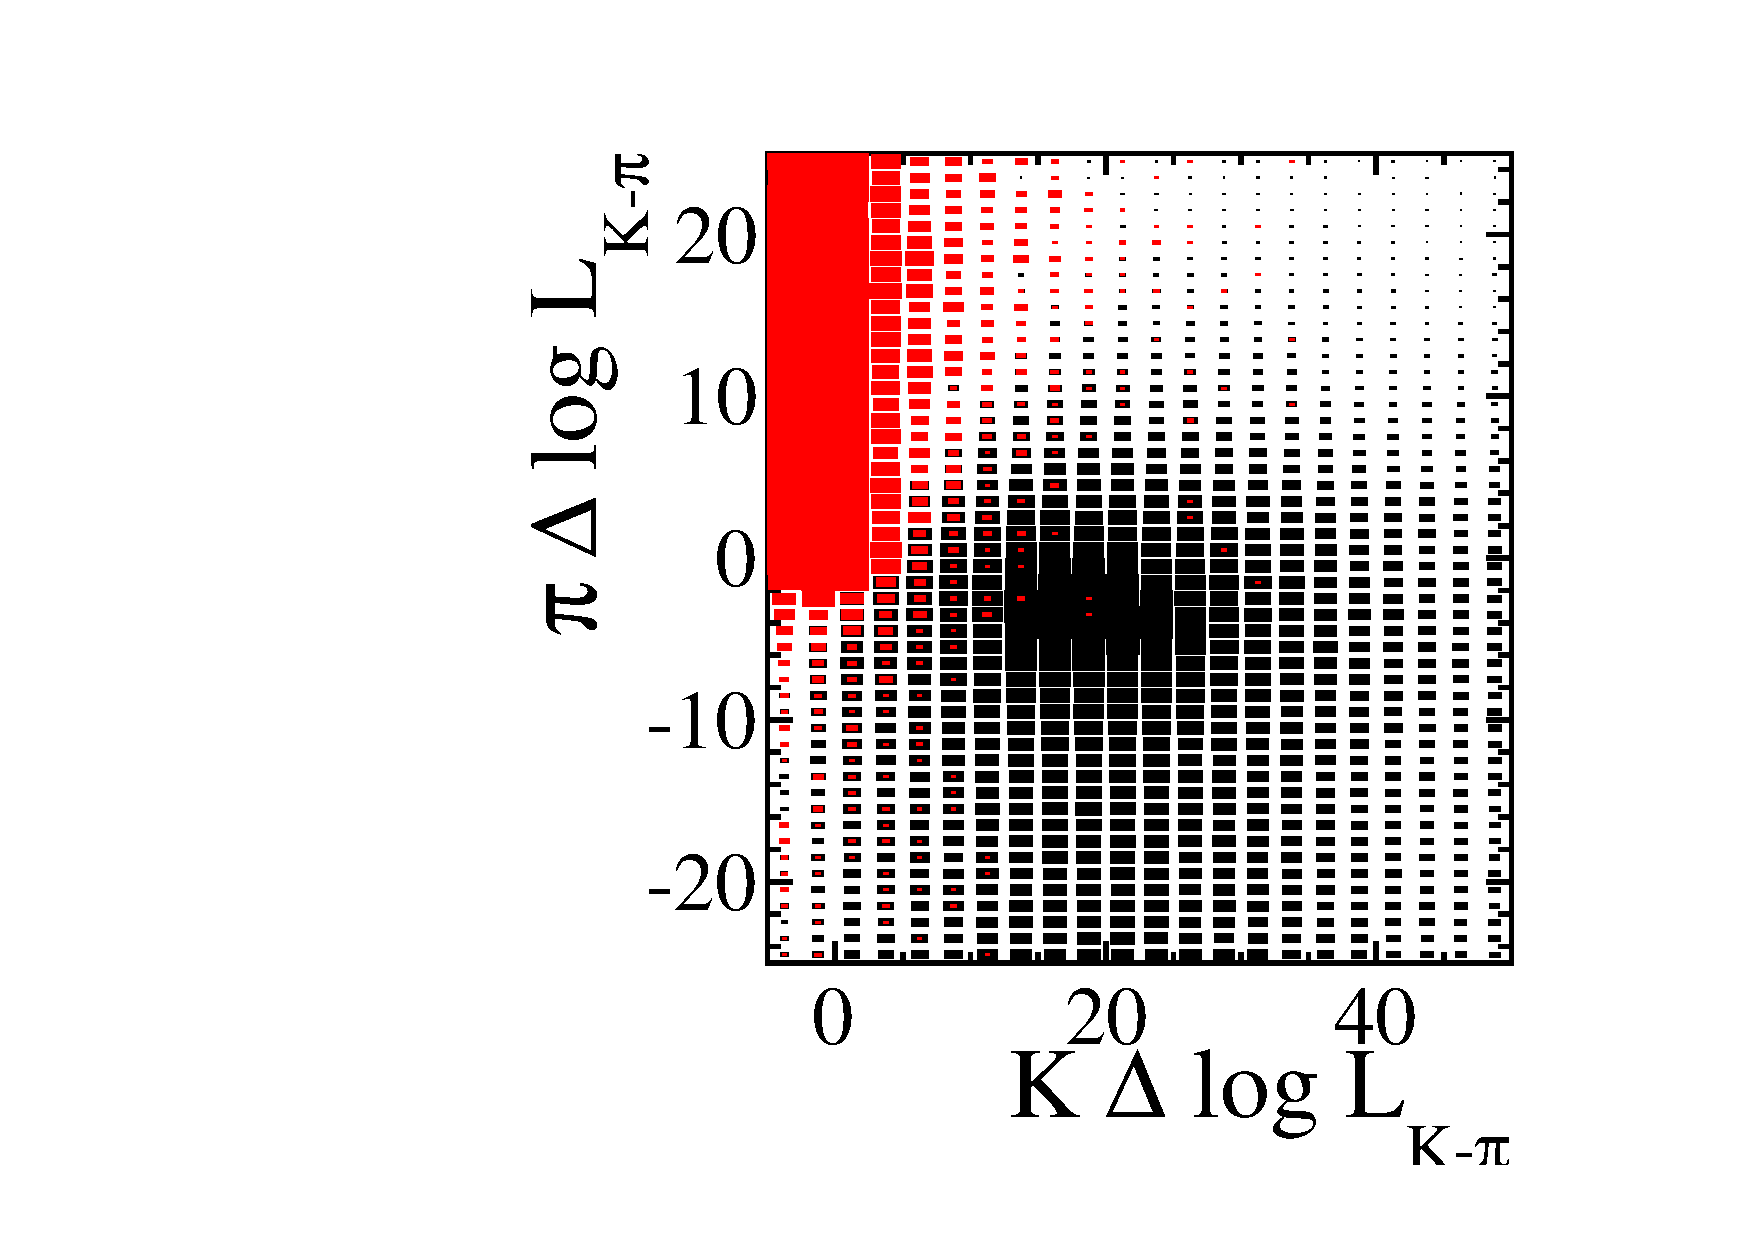
\includegraphics[width=0.48\columnwidth]{chapter7/figs/kstarmumu_swap_2Ddist.pdf}
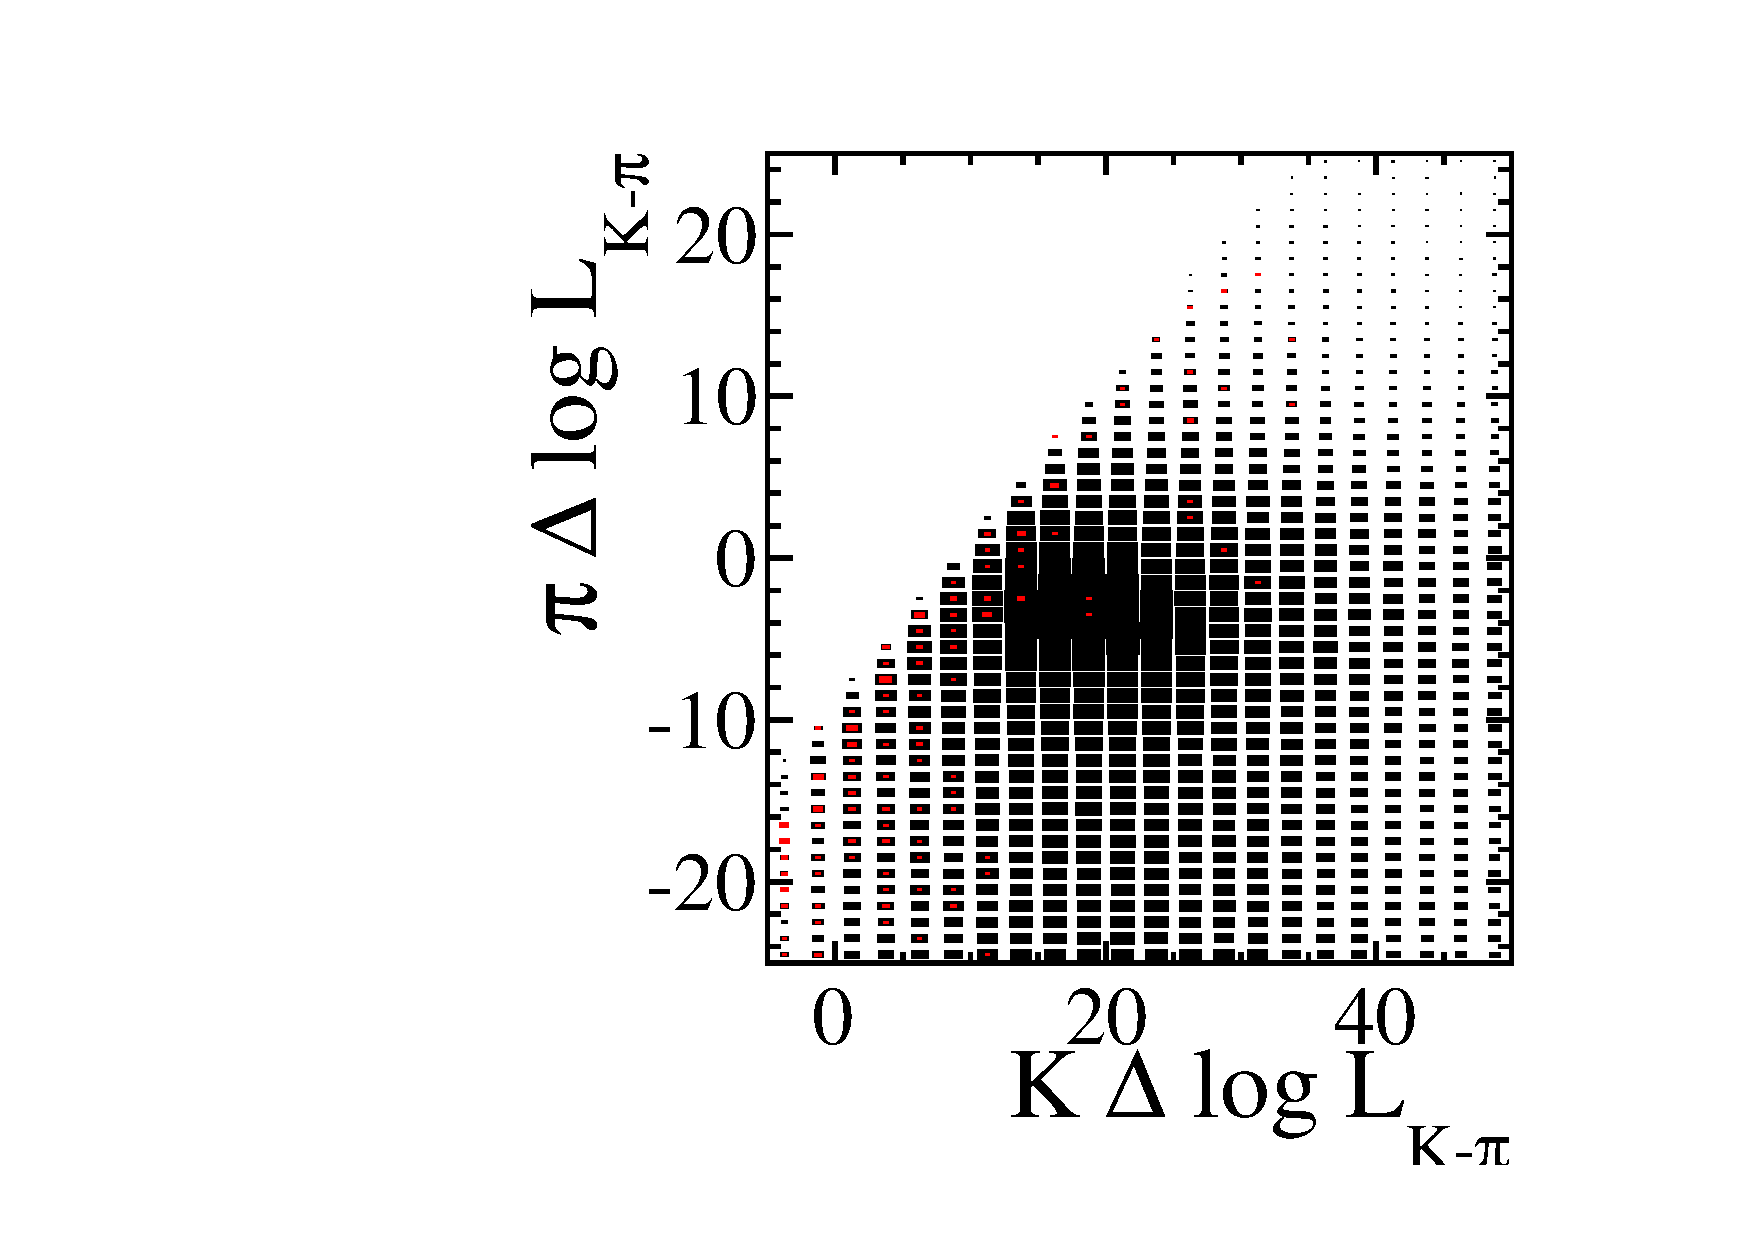
\includegraphics[width=0.48\columnwidth]{chapter7/figs/kstarmumu_swap_2Ddist_veto.pdf}
\caption[  The distribution of \BdToKpimm simulation (a) before and (b) after the \ktopi swap veto.   ]
{The distribution of \BdToKpimm simulation (a) before and (b) after the \ktopi swap veto. 
Candidates with the correction assignment of masses for the kaon and pion are shown in black and candidates 
with the incorrect assignment of masses are shown in red. There is a clear overlap of candidates around \dllkpi of 0 for both particles.
~\label{fig:swave:meas:kpiswaps} }
\end{figure}
The overlap of the two distributions can be seen around the zero point motivating the use of the diagonal cut, $\kdllkpi-\pidllkpi>10$.
The efficiency of the swap veto is around 92\% on signal events which pass the multivariate selection and 
less than 2.5\% of swapped candidates are retained after the veto.
There are less than 0.1\% of \ktopi swap candidates in the simulation after selection.

\subsubsection{Other peaking backgrounds}

The possible sources of peaking backgrounds considered have a % are also considered in Section~\ref{sec:kstmm:sel} and
mass close to the \Bd mass after the misidentification of one or more of the final state particles
 and could create structure in the \kpi mass spectrum. They are
\begin{itemize}
\item \BdToKstmm with the pion misidentified as the muon and the muon as the pion.
\item \BdToKstmm with the kaon misidentified as the muon and the muon as the kaon.
\item \BsToPhimm with one of the kaons misidentified as a pion.
\item \BuToKmm with an added soft pion.
\item \LbToLmm (1) with the proton misidentified as a pion.
\item \LbToLmm (2) with the proton misidentified as a kaon and the kaon misidentified as a pion.
\end{itemize}
In order to understand the \kpi mass distribution of these exclusive backgrounds, 
simulation samples for each decay were used. % generated and corrected as described in Section~\ref{sec:kstmm:data:mccorr} .
Each simulation sample was weighted so that the number of events in the sample was equivalent to the expected yield from 1.0\invfb of data.
The number of events after selection for the signal \Bd and \kpi mass region, the signal \Bd and the wide \kpi mass region
 and the wide \Bd and the wide \kpi mass region are shown in Table~\ref{tbl:peaking:backgrounds}.
\begin{table}
\centering
\caption[   The expected number of peaking background events from selected simulated data in three different mass ranges
for an integrated luminosity of 1.0\invfb.   ]
{ The expected number of peaking background events from selected simulated data in three different mass ranges
for an integrated luminosity of 1.0\invfb. The assumed branching fraction is given in the first column.
The first mass range is from $5230<\mB<5330\mevcc$ and $800<\mkpi<1000\mevcc$. 
The second mass range is from $5230<\mB<5330\mevcc$ and $634<\mkpi<1200\mevcc$ 
The third range mass range is from $5200<\mB<5700\mevcc$, $634<\mkpi<1200\mevcc$. 
The errors are statistical.~\label{tbl:peaking:backgrounds} }
\begin{tabular}{|c|c|c|c|c|}
\hline
Background  & $\Gamma$  & Range 1 & Range 2 & Range 3 \\
\hline
\BdToKstmm ( $K\leftrightarrow\pi$ )  &   $1.0\times10^{7}$&  $ 0.119\pm0.345 $ &$ 0.158\pm0.397 $ &$ 0.487\pm0.698 $ \\ 
\BdToKstmm ( $\pi\leftrightarrow\mu$ )  & $1.0\times10^{7}$&  $ 0.5\pm0.707 $ &$ 1.5\pm1.22 $ &$ 2.33\pm1.53 $ \\ 
\BdToKstmm ( $K\leftrightarrow\mu$ ) &    $1.0\times10^{7}$&  $ 0\pm0 $ &$ 0\pm0 $ &$ 0\pm0 $ \\ 
\BsToPhimm  &                             $5.5\times10^{7}$&  $ 3.1\pm1.76 $ &   $ 5.93\pm2.44 $ &$ 7.91\pm2.81 $ \\ 
\BuToKmm  &                               $6.0\times10^{7}$&  $ 0.0851\pm0.292 $ &  $ 0.17\pm0.413 $ &$ 1.3\pm1.14 $ \\ 
\LbToLmm (1)  &                           $1.0\times10^{7}$&  $ 13.2\pm4.63 $ &   $ 25.1\pm7.01 $ &$ 79.7\pm10.93 $ \\ 
\LbToLmm (2) &                            $1.0\times10^{7}$&  $ 3.8\pm2.95 $ &$ 6.82\pm3.61 $ &$ 13.3\pm5.64 $ \\  
\hline
\end{tabular}
\end{table}
%As measured in Section~\ref{sec:kstmm:res}, there are 900 \BdToKstmm candidates in the 1.0\invfb data. 
%This means that most of the peaking backgrounds are around 1\% or less in the signal region, 
%justifying their ignorance in the previous measurement.
%However, there are larger contributions from the peaking backgrounds in the high \kpi mass region and the higher \Bd mass region.
The distribution of peaking background simulation is given in figure~\ref{fig:swave:peaking:backgrounds}.
\begin{figure}
\centering
\subfigure[]{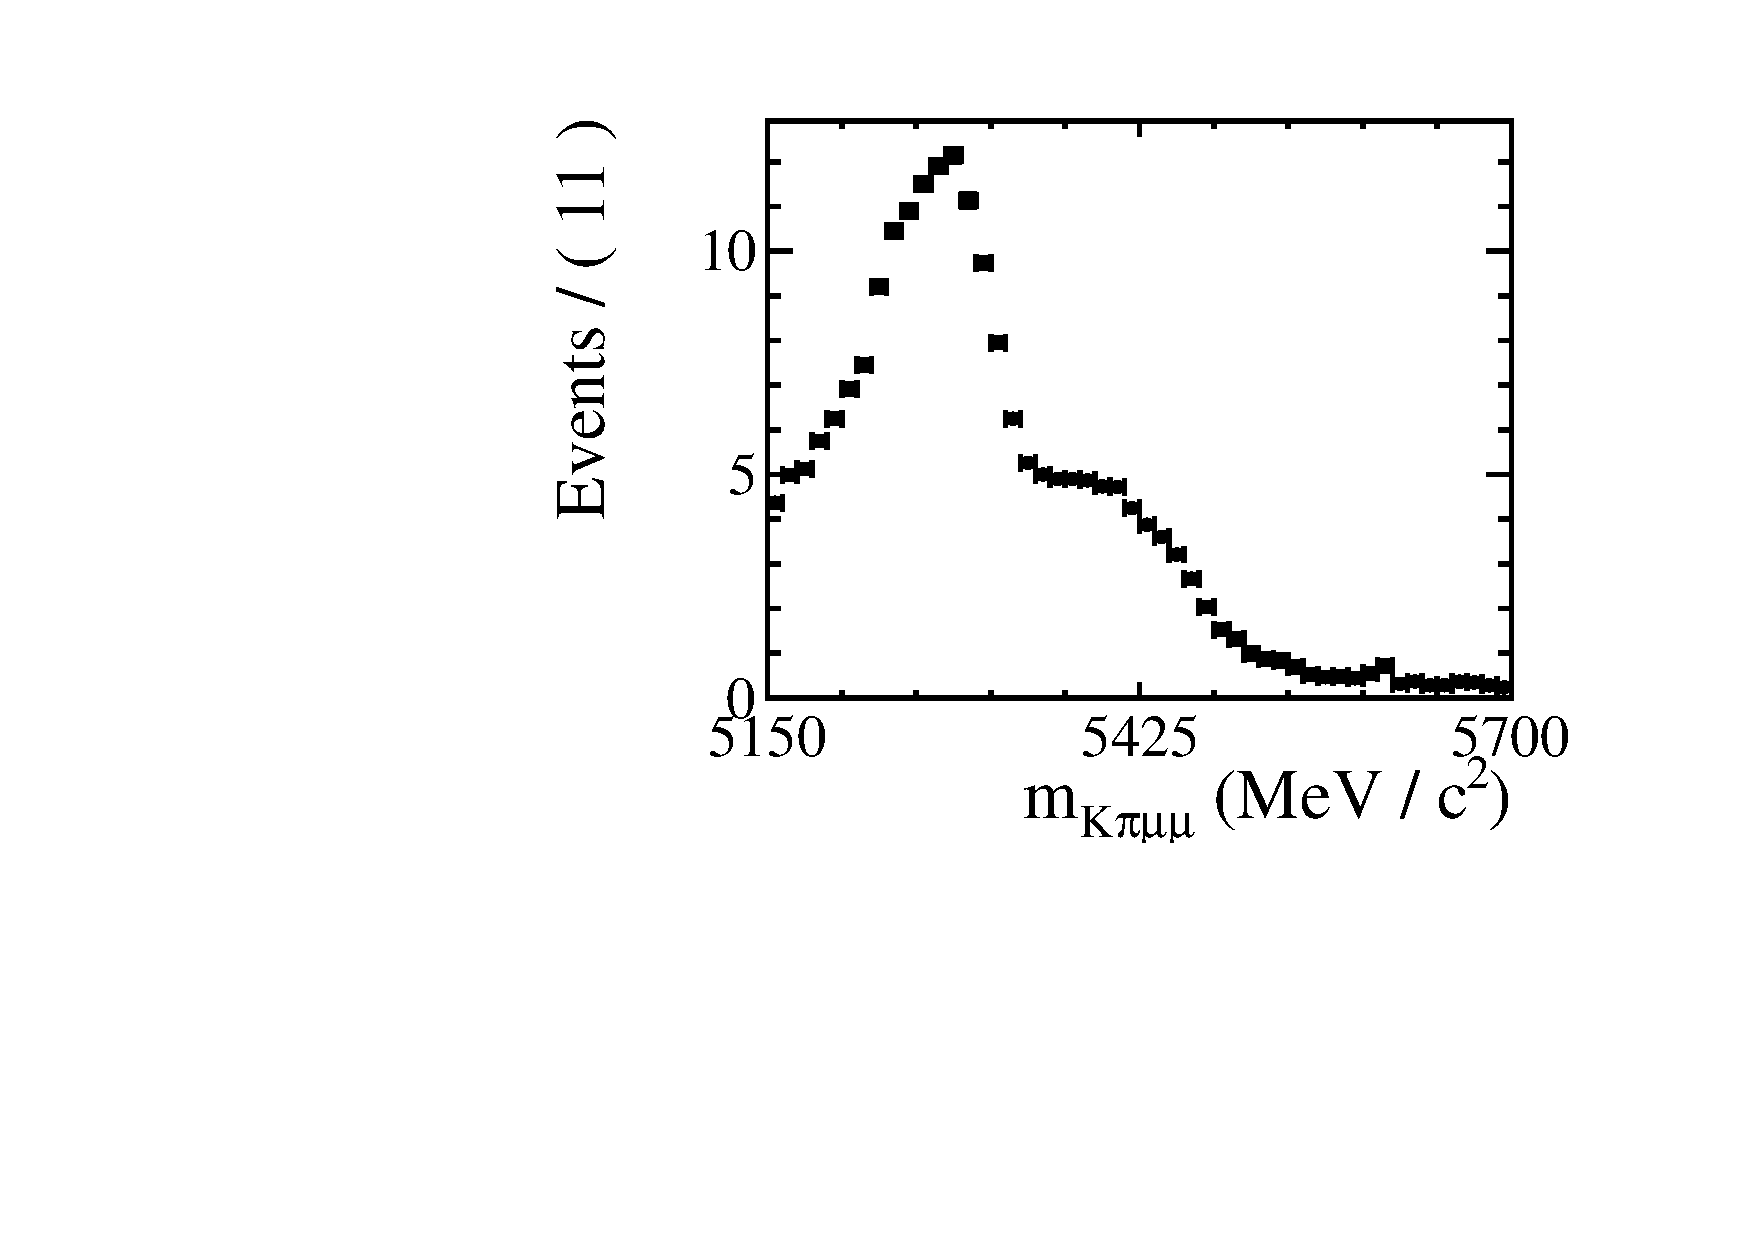
\includegraphics[width=0.32\columnwidth]{chapter7/figs/peaking/peaking_backgrounds_mass.pdf}}
\subfigure[]{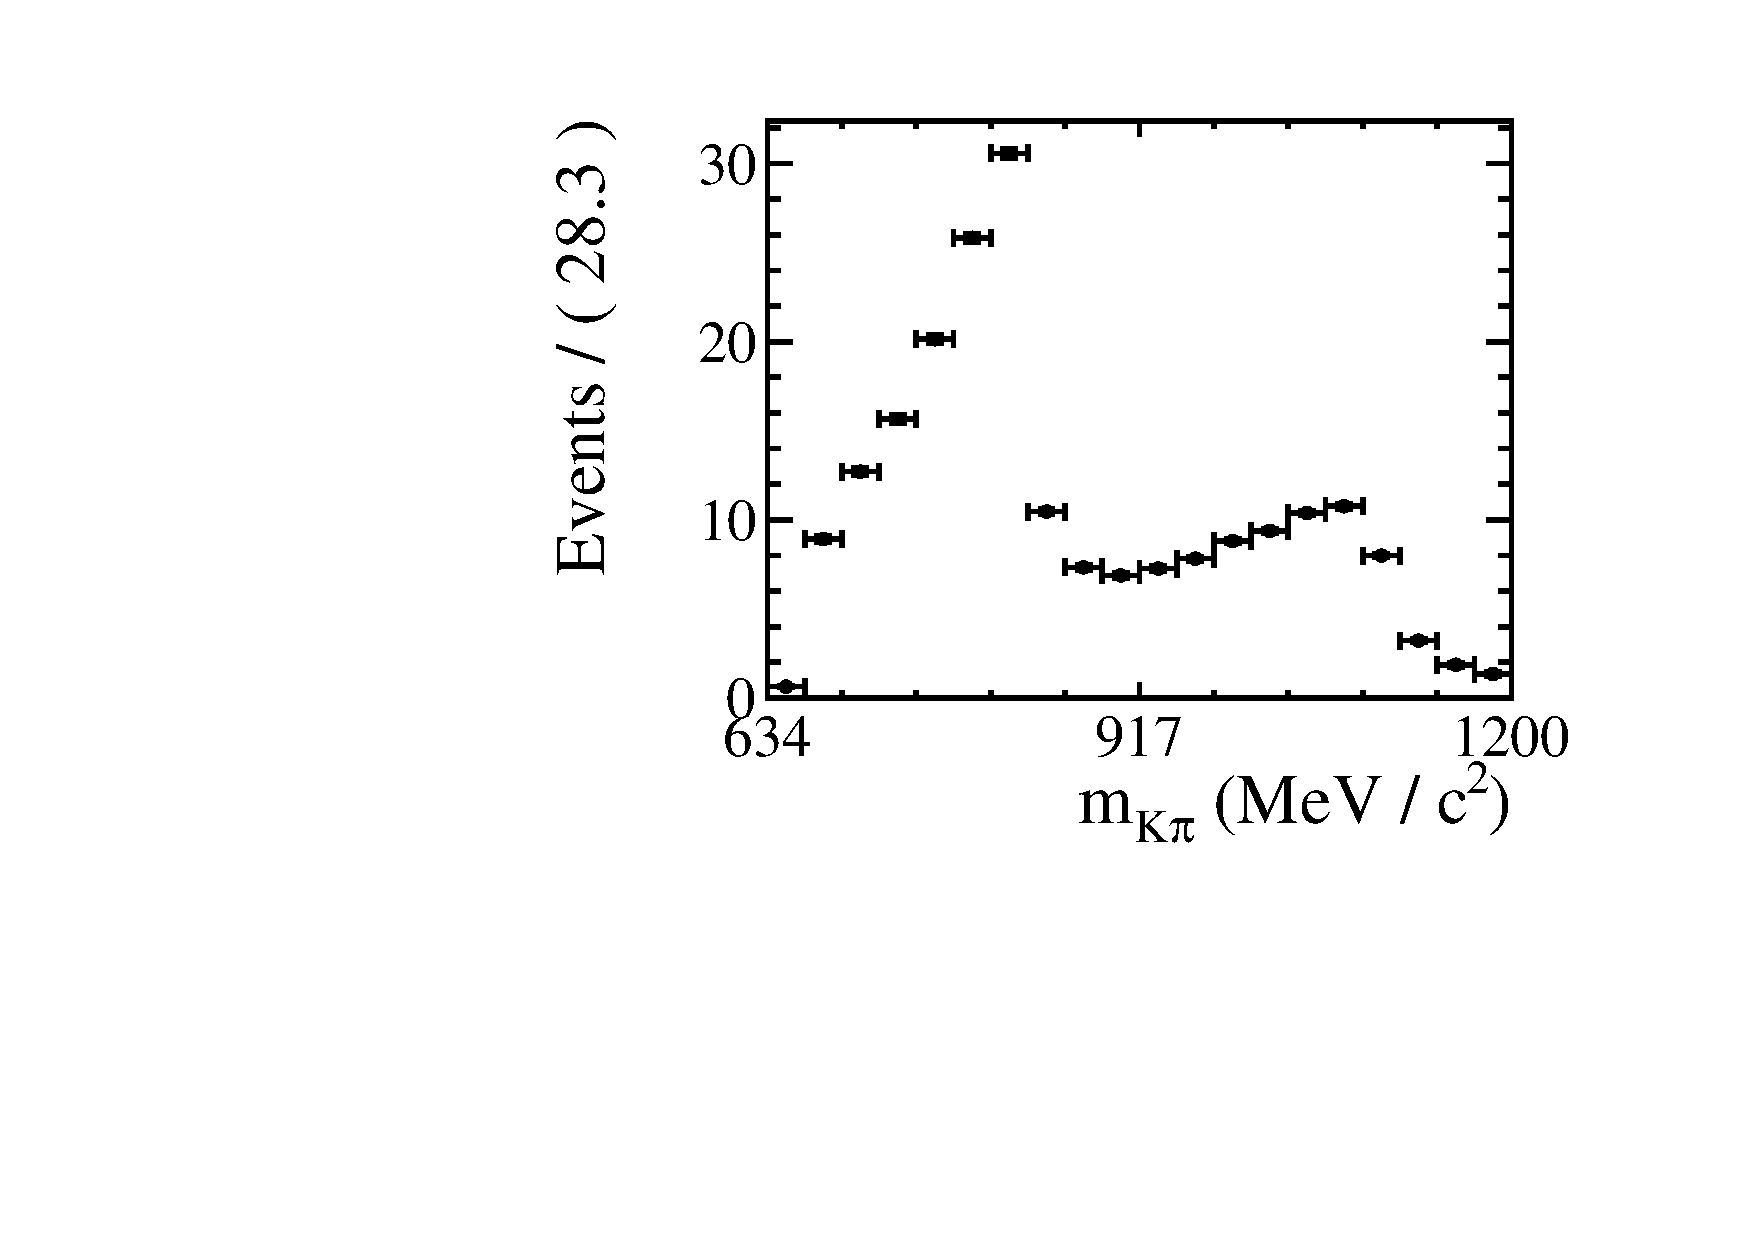
\includegraphics[width=0.32\columnwidth]{chapter7/figs/peaking/peaking_backgrounds_mkpi.pdf}}
\subfigure[]{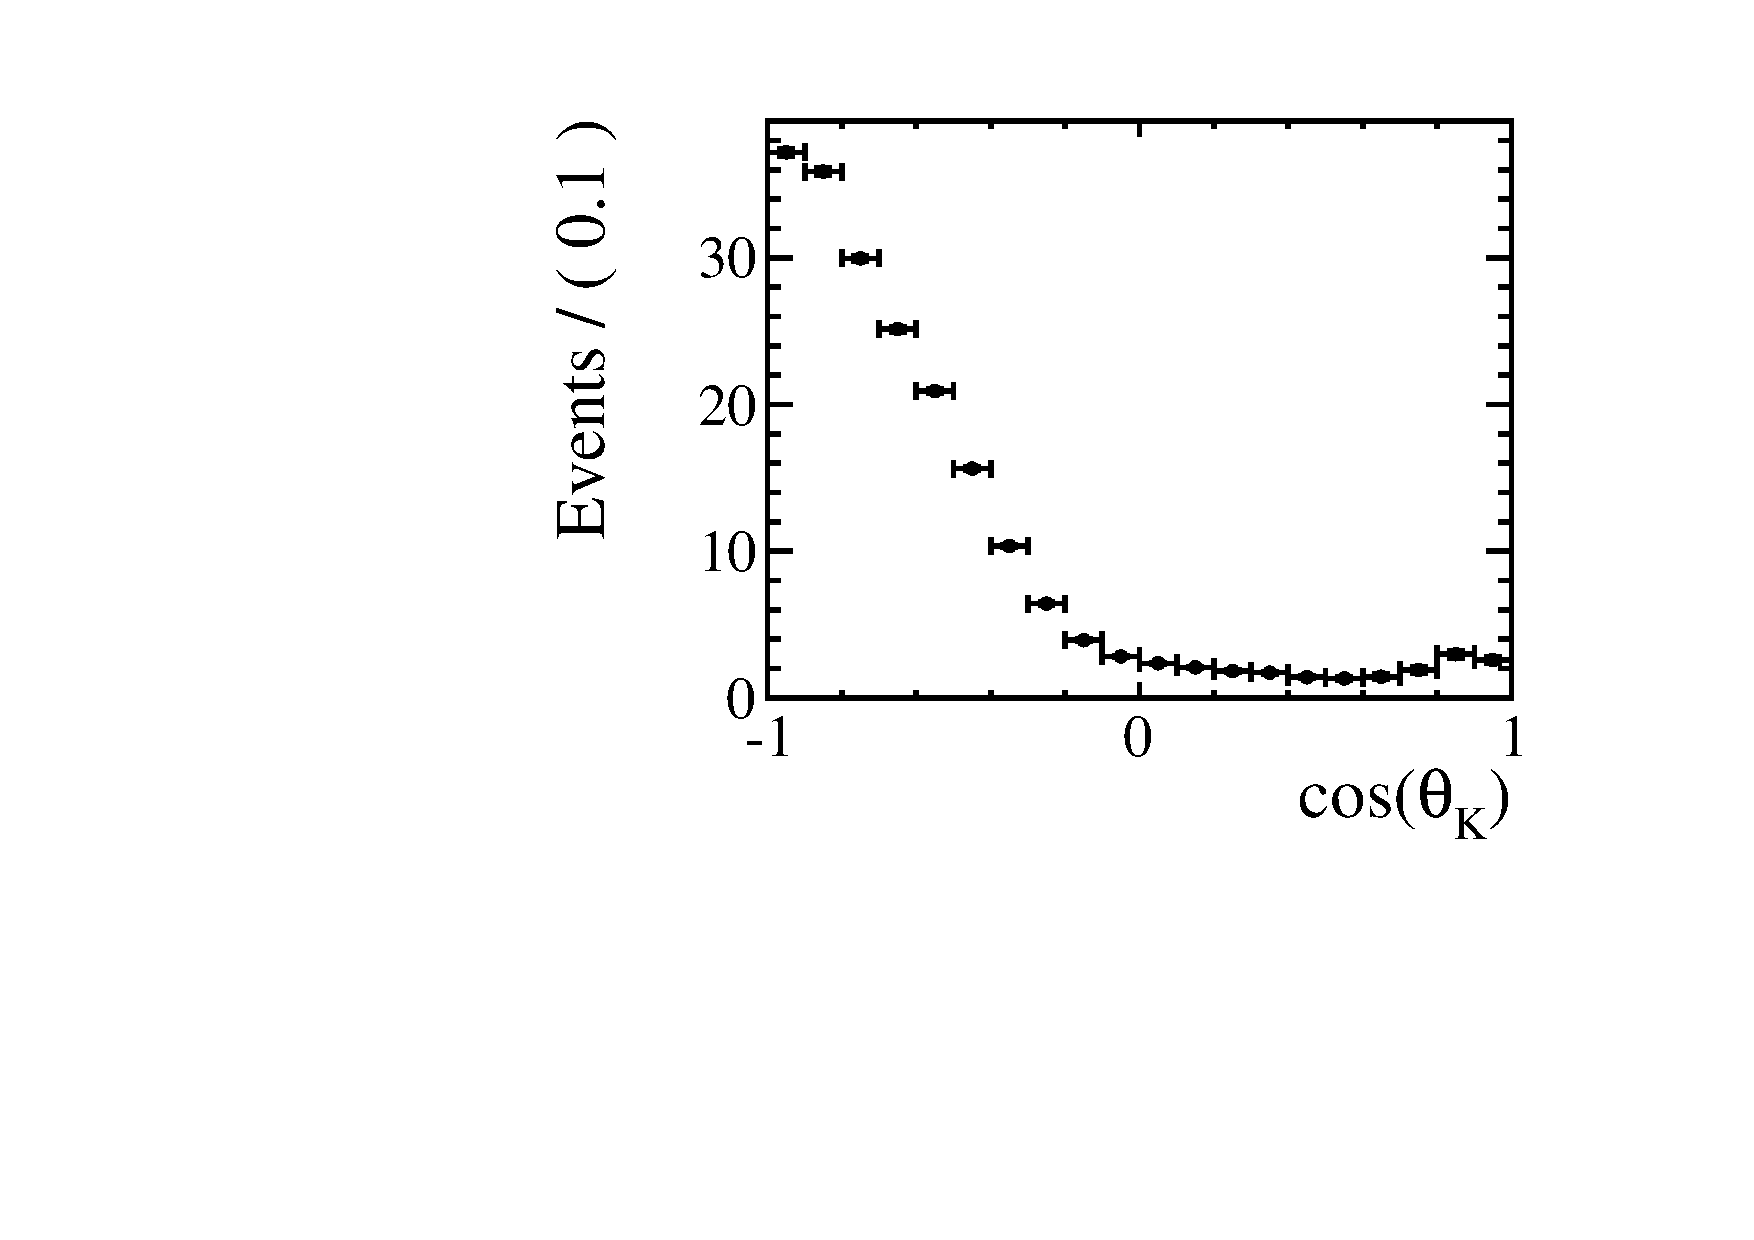
\includegraphics[width=0.32\columnwidth]{chapter7/figs/peaking/peaking_backgrounds_ctk.pdf}}
\caption[ The combined distribution of peaking background events after selection in terms of (a) \mkpimm, (b) \mkpi and (c) \ctk.   ]
{ The combined distribution of peaking background events after selection in terms of (a) \mkpimm, (b) \mkpi and (c) \ctk.
The distribution is composed of simulated \BdToKstmm, \BsToPhimm, \BuToKmm and \LbToLmm normalised to
the expected number of events in 1.0\invfb of data. %It is possible to see non-trivial shapes 
%in the \kpimm and \kpi mass distributions.% but the number of events is almost insignificant.
~\label{fig:swave:peaking:backgrounds} }
\end{figure}
It is possible to see structure in each of the \mkpill, \mkpi and \ctk distributions.
However, the fraction of peaking background events in the \kpill mass window is less than $(2.0\pm0.2)\%$ after the selection allowing these contributions to be ignored under the P-wave peak.

%\subsection{Data distributions}
%The distribution of selected \BdToKpimm and \BdToJpsiKpi candidates as a function of \mB and \mkpi are shown in Fig.~\ref{fig:swave:mass:mkpi}.
%Here the \mkpi window is extended upwards to 2000\mev to show the overall distribution of events at high \mkpi.
%\begin{figure}[tbp]
%\centering
%\subfigure[]{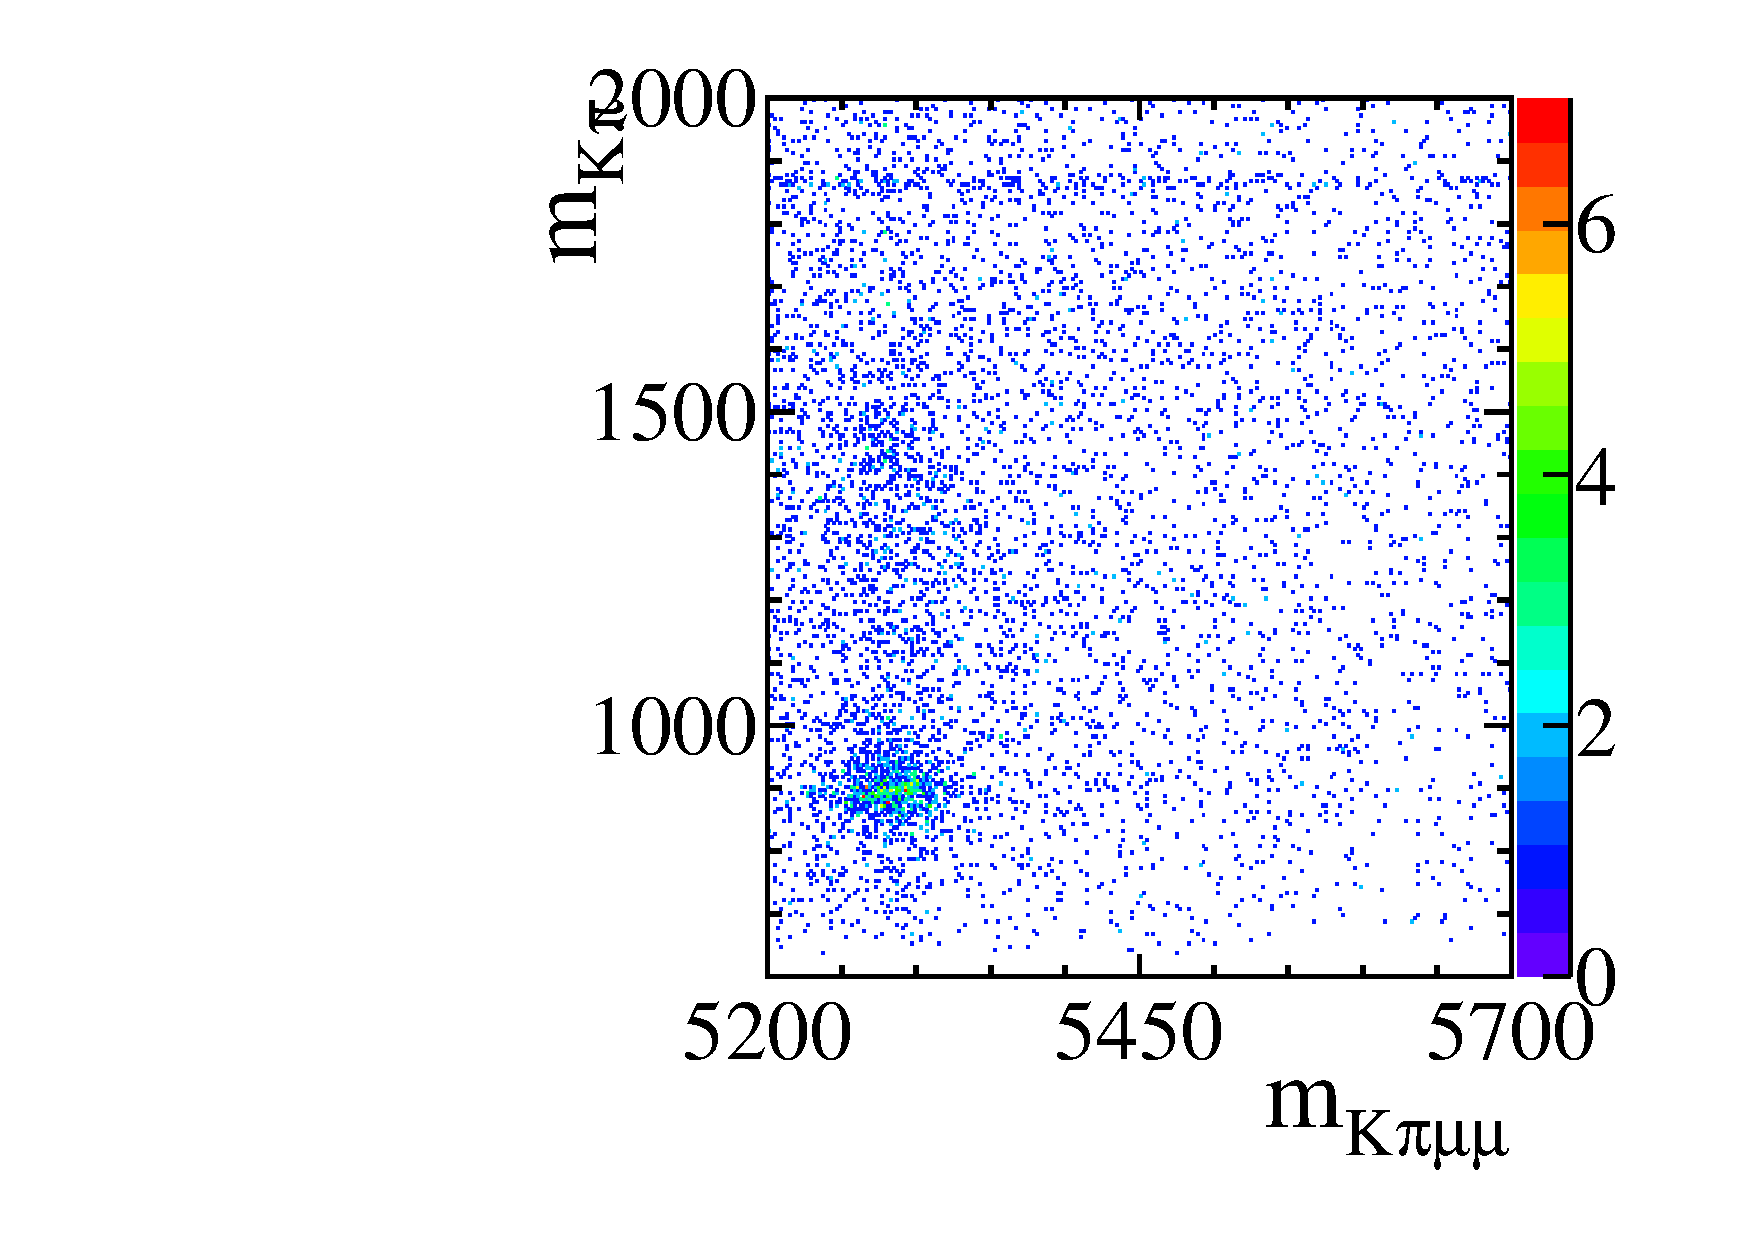
\includegraphics[width=0.48\columnwidth]{chapter7/figs/massdists_kstarmumu_mB_mkpi.pdf}}
%\subfigure[]{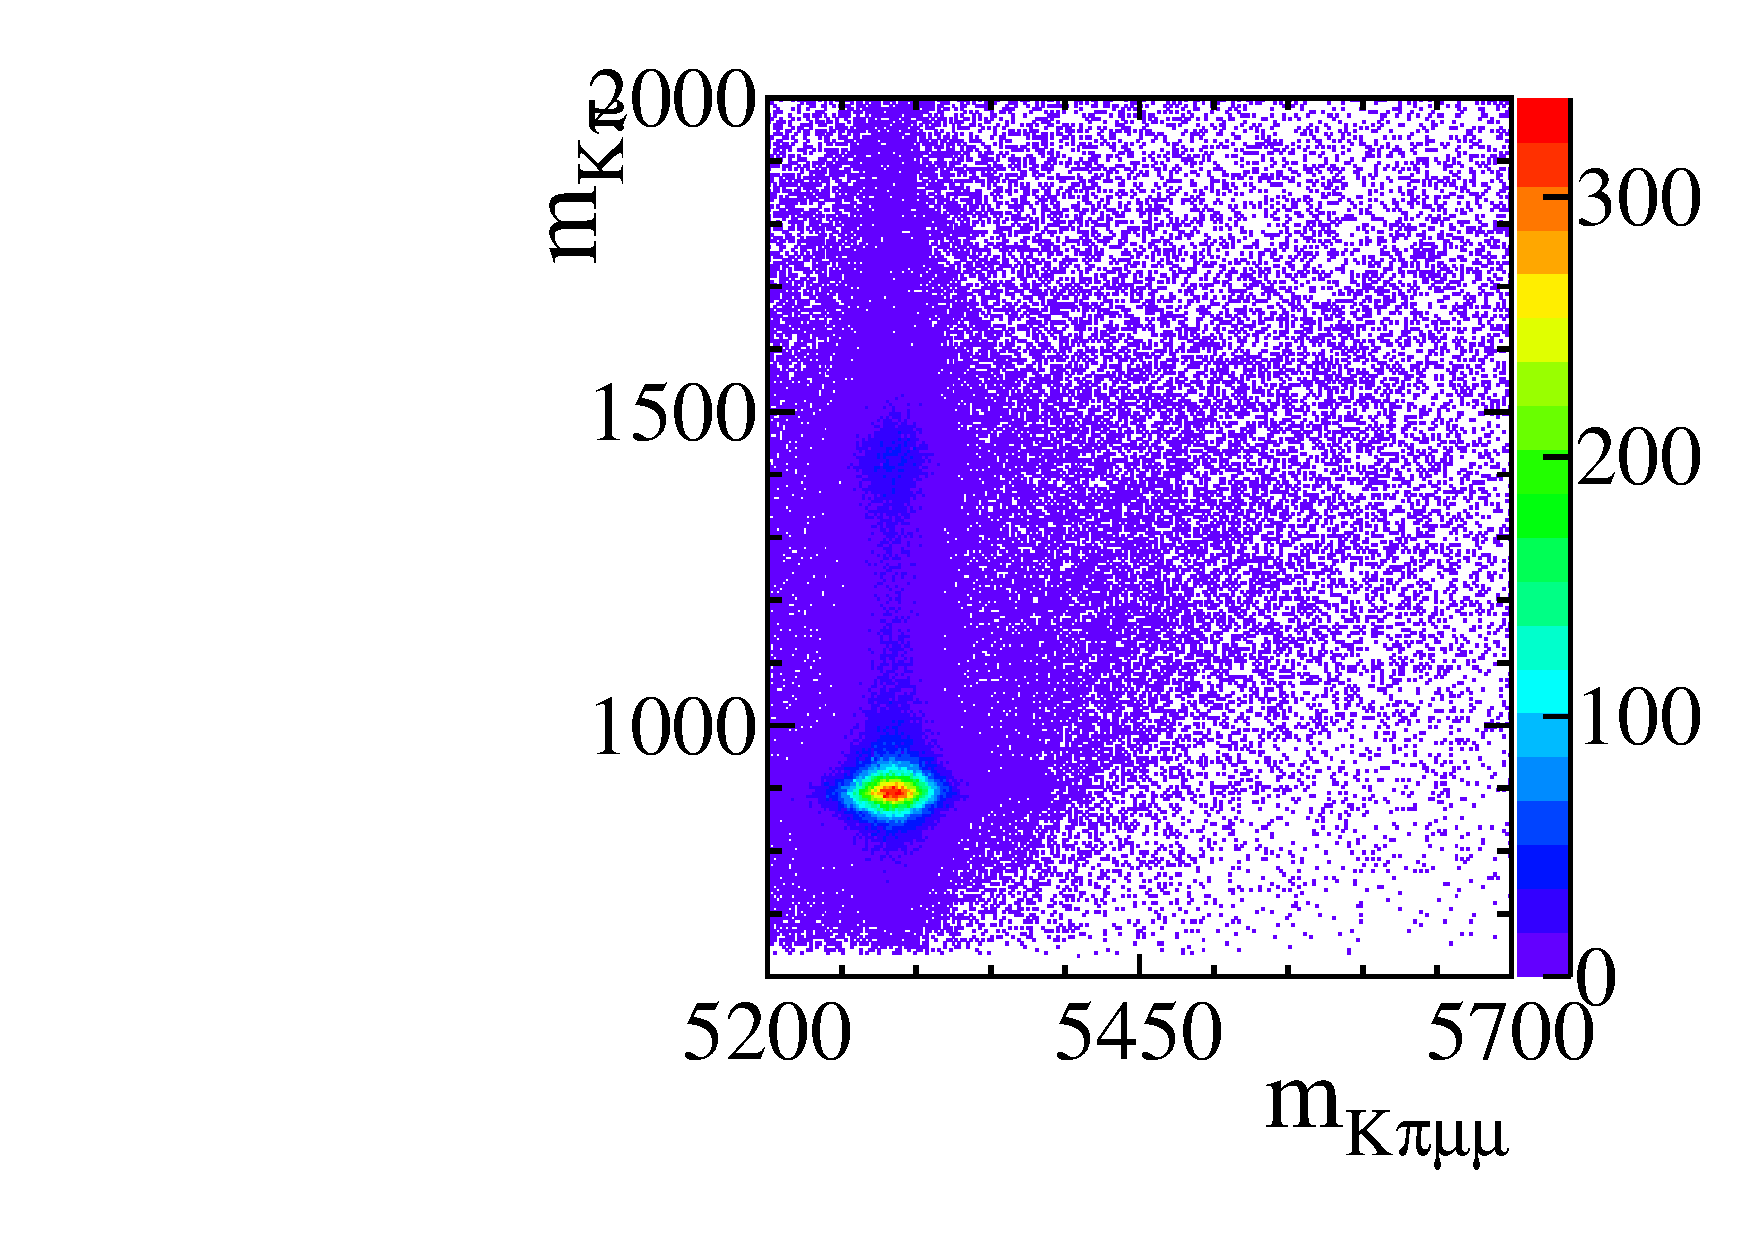
\includegraphics[width=0.48\columnwidth]{chapter7/figs/massdists_jpsikstar_mB_mkpi.pdf}}
%\caption{ \mB v.s. \mkpi mass distributions for the wide \mkpi region for (a) \BdToKstmm and (b) \BdToJpsiKstar. 
%In the \BdToKstmm selection, it is possible to see the P-wave clearly and a 
%combinatorial background from \D \mumu at $\mkpi\sim1800$.
%In the \BdToJpsiKstar selection, is it possible to see both the P-wave, the \kpi S-wave and a \Kstarz D-wave at 1430.
%There is also an asymmetric background in \mkpi and \mB. ~\label{fig:swave:mass:mkpi} }
%\end{figure}
%It is possible to see a clear peak of \BdToKstmm events along with a generic S-wave and 
%contributions from the $\Kstarzt(1430)$ in the \BdToJpsiKpi spectrum as described in Ref~\cite{LHCB-PAPER-2012-014}.
%There is significant difference between the high \mB background between \BdToJpsiKpi and \BdToKpimm.
%The background for the charmonium mode can be seen in increase with \mkpi indicating that it is mis-reconstructed physics background whereas the 
% \BdToKpimm background is constant as a function of \mkpi indicating that it is composed of mostly combinatorial background.




